\documentclass[11pt,a4paper]{article}
%\usepackage[spanish]{babel}
\usepackage[utf8]{inputenc}
\usepackage{amsmath}
\usepackage{amsfonts}
\usepackage{amssymb}
\usepackage{graphicx}

\pagestyle{empty}
\setlength\parindent{0pt}

\addtolength\topmargin{-1cm}
\addtolength\textheight{2cm}
\addtolength\textwidth{2cm}
\addtolength\oddsidemargin{-1cm}
\begin{document}

\begin{center}
{\LARGE \textbf{Computer Vision-based hand\\gesture recognition\\}}
\vspace{0.2cm}
CSCI 5109 Visualization\\
César Mora Castro\\
\textit{castr148@umn.edu}\\
\end{center}
\vspace{1cm}


%% ========================================
%%  MOTIVATION
%% ========================================

\section{Motivation}
The main motivation of this project is the opportunity to put into practice my knowledge and passion about Computer Graphics and Computer Vision with the techniques and principles about flow visualization acquired in this class.\\

Flow data can be obtained from many different sources: fluid flows (water, blood, air), electric or magnetic fields,  heat maps, force maps, etc. A video stream (taken from a web cam, for example) is nothing more than a succession of numbers continuously flowing, and from which a lot of important features can be extracted. In this sense, the main purpose of Computer Vision is to develop algorithms that can obtain those features: identify faces of people, recognize objects or predict suspicious behaviors.\\

In the past, I acquired experience working with Augmented Reality algorithms, that detect markers, image features and visual descriptors in order to estimate the camera pose and render virtual objects directly over the real scene. However, I did not have a significant amount of experience developing my own algorithms to artificially detect a complex behavior.\\

For these reasons, I propose the development of an  algorithm to detect the hand gestures, in real time, from a video stream. I will not use any high-level library to do it, but I am going to relay in the basics imaging algorithms provided by the open source library \textit{OpenCV}. Moreover, I prefer the algorithm to be more autonomous and scalable than efficient, although optimizations are going to be really important during the whole process.\\

The most important goals that I have proposed for this project are:
\begin{itemize}
\item The system should be autonomous and independent. It is desirable to have the least amount of pre-training or training required per execution as possible.
\item It should work with (almost) any background and illumination configuration possible (within a reasonable scope).
\item Use multi-platform dependencies, to make it easily portable to other operating systems.
\item Design it as a \textit{library}, so that other applications can use it to incorporate gesture recognitions.
\item Make it modular, to easily incorporate different skin tonalities and gestures.
\end{itemize}
 
Given that this is a project with a due date, it was difficult to estimate what features will be fully implemented, since these are algorithms that are not completely solved. Also I wanted to have some kind of \textit{freedom} designing the algorithm, to get room for testing different methods and techniques.\\

Without further ado, here are the results that I achieved.\\

%% ========================================
%%  LITERATURE REVIEW
%% ========================================

\section{Literature Review}

Before start working on the code of this project, I performed a literature review to know better the existing approaches and techniques that solve this challenge.\\

In the beginning, I started by reading the articles \textit{Vision-based gesture recognition: A review}~\cite{wu1999vision}, by Y. Wu, and \textit{Computer vision-based gesture recognition for an augmented reality interface}~\cite{storring2004computer}, by M. Storring. With these articles, I learned the basics of image segmentation, histogram selection to identify certain \textit{textures}, and contours moments to measure the similarity between two shapes. However, I did not want to follow a specific  pre-existing algorithm, but instead try to come up with my own after experimenting with different techniques. In fact, in the next section I do not only explain the final implementation, but the whole path followed during the development along with strengths/weaknesses encountered.\\

The next logical step was the studying and learning the capabilities of the library \textit{OpenCV}. The documentation of the \textit{API} can be found in \cite{OpenCVdoc2013}, along with multiple really useful tutorials. \textit{OpenCV} is divided in different modules, in charge of different operations (image operations, objects tracking and matching, video stream controller, etc). This way it is easier to explore the algorithms provided.\\

%% ========================================
%%  PROJECT
%% ========================================

\section{Project}
The Figure \ref{general_scheme} shows the block diagram of the overall system. The main classes that perform the detection and recognition of the gesture are \textit{Hand Detector} and \textit{Gesture Recognizer}:\\

\begin{figure}[tbh]
\centering
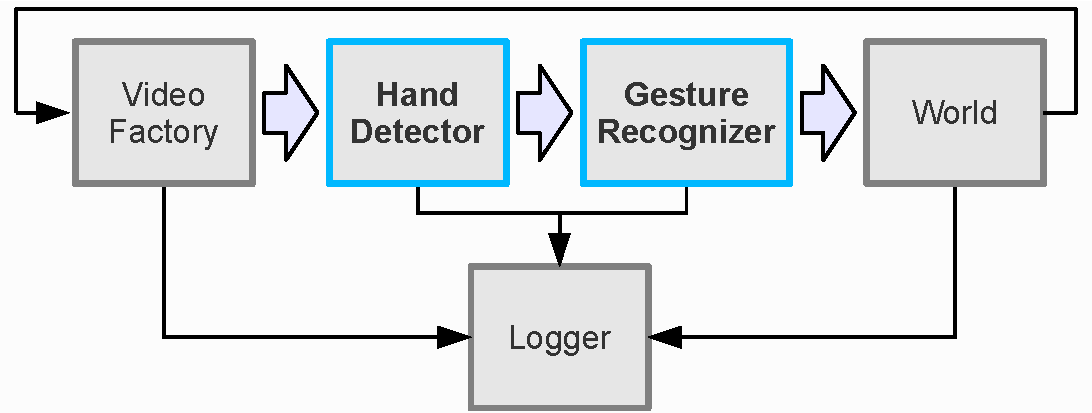
\includegraphics[width=13cm]{images/general_scheme}
\caption{Block diagram of the system.}
\label{general_scheme}
\end{figure}


\begin{itemize}
\item \textit{HandDetector takes as input one unique frame, and returns an array of masks (binary images) of the detected hand, with different configurations (skin histograms).}
\item \textit{GestureRecognizer takes as input the array of masks, and returns the gesture recognized (if any).\\ }
\end{itemize}

The rest of the classes are supportive of this ones to provide them basic functionality. We will start by explaining the latter classes, and afterwards we will go into detail about the two main classes.

\subsection{VideoFactory}
This class only implements a Factory to provide \textit{VideoSource}. Is is designed to keep track of more than one video source, but in this case it is only one necessary.

\subsection{World}
This \textit{inaccurately}-called class its in charge of basic drawing and management operations. The following is a detailed description of the most important tasks that this class performs:
\begin{itemize}
\item Control of the timing of the algorithm. It tries to keep a constant user-defined amount of \textit{FPS} (Frames per second).
\item Initialize and manage the result windows. The application shows one \textit{OriginalFrame} window (shows the frame as it is grabbed from the camera), one \textit{ResultWindow} (shows the contour of the recognized gesture, if any), and six \textit{TestWindows}. The latter are used to show intermediate results of the algorithm (segmentation, blur, flood operations, erosion, etc).
\end{itemize}


\subsection{Logger}
This \textit{Singleton} class writes log messages (notes, warnings or errors) into a text file.

\subsection{HandDetector}
This class takes a frame as an input, and returns an array of masks (as many as skin histograms are available). This means that tries to detect the hand according to different kinds of skins colors and illuminations. The Figure \ref{hand_detector} shows the block diagram of the algorithm. The following is the description, step by step, of this algorithm, explaining the process followed until this final approach was adopted.\\


\begin{figure}[tbh]
\centering
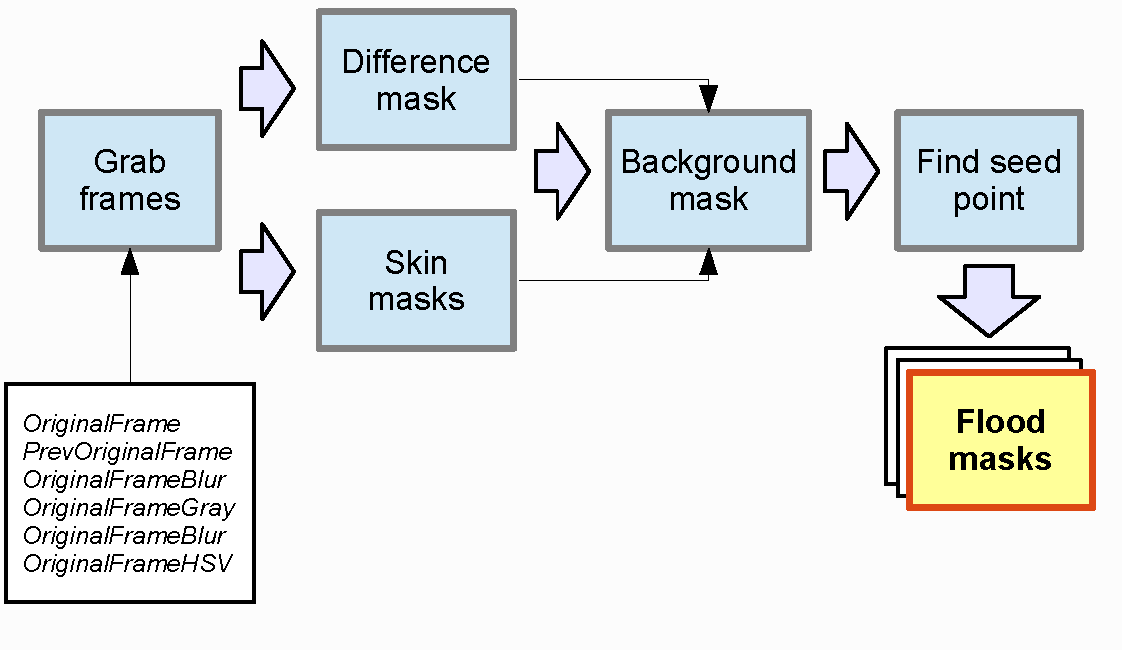
\includegraphics[width=13cm]{images/hand_detector}
\caption{Block diagram of the hand detector.}
\label{hand_detector}
\end{figure}

\begin{itemize}

\item When it is created, the \textit{HandDetector} loads the histogram files. It will try to load as many files as it can find, with the name \textit{histogramX.yml}, which \textit{X} is a number starting in 1.

\item The algorithm fetches a frame from the camera. It resizes it, since a full resolution frame is not needed (and the computations are less expensive), and converts it into different formats. These conversions are shown in the Figure \ref{hand_detector}. The \textit{blur} effect is applied to get more smoother results, and to remove some noise from the image (this makes the results from different continuous frames smoother). Some methods uses one channel images, so the Gray scale version is often used. The HSV version of the image is used in order to get the skin histograms, since they are better to represent than the RGB one. Also, the previous frame is also stored, to create a \textit{motion difference} map.

\item Get the difference mask. To get this mask, first the algorithm gets the difference frame between the current frame and the previous one. This difference frame is computed with the function \textit{absdiff}. Then it applies a threshold function to get the mask. The threshold is defined by the constand \textit{THRES\_DIFF\_MASK}.\\

At first, in order to calculate the \textit{movement} of the frame, I used an optical flow algorithm. This algorithm searched for feature points in the image and calculated the movement vector of them. However, the need of this system is to know \textit{where is movement, no matter how}, which is easier than a complex optical flow algorithm (which identifies features and where they are moving). Calculating a difference map turned out to be more efficient and effective, since it gives better results.

\item Get the skin masks. For each skin histogram, the algorithm gets a skin mask. This is computed by the function \textit{calcBackProject}, which calculates the back projection for that histogram. This projection just creates a one-channel frame indicating the probability of each pixel of belonging to that histogram. Then, a threshold function is applied with threshold defined by the constant \textit{BACK\_PROJ\_THRES}.\\

In a first approach, I did not use the back projection technique to get the skin mask. I analyzed, manually, each component H, S and V of different skins and illumination conditions, and I tried to get a range of values that corresponded to skin. The major shortcoming is that this range of values where unique for each component (defined by a max and min value). With the histogram approach, this can be specified with a more accurate and complex way.

To calculate the skin histograms, I developed another tool. This tool also creates the gesture files, and it is described in the section \ref{tool}.

\item Once the algorithm has calculated the difference mask and the skin masks, for each skin mask it does the following:
	\begin{itemize}
	\item Join the difference mask and the skin mask with an \textit{OR} operation. This new mask represent places that are likely to be skin (it is moving and it has skin color).

	\item The algorithm uses an accumulator to extract the background. Every frame is \textit{accumulated}, so the pixels that do not move are considered to be part of the background. The algorithm gets a mask from this accumulator. It subtracts from the actual frame the background accumulator. This so called background mask represent parts that are from the background. The last mask (sum of skin and difference mask) is used when accumulating a new frame: parts that are likely to be skin are not accumulated, since they do not belong to the background.
	
	\item The background mask is eroded, to remove more noise. This causes the mask to be cleaner (small spots that are identified as skin are deleted, since they are too small to be a hand).
	
	\item In order to identify the hand mask (the one that only represents the hand) it is necessary to find the \textit{seed point}, a point belonging to the hand. This is more tricky than it seems at first, because there would be other parts of the background that can be confused with skin, or the proper face of the user. This point is found in two ways.\\
	
	The first step, is finding the seed point in the difference map. This is, if there is a part of the image that is moving (with a considerable speed), and that part has skin color (belongs to the skin map), then the algorithm identifies as the seed point.\\
	
	If this step does not success in finding a seed point (just because the hand is not moving), the system tries to find it by \textit{interpolation}. This means that it takes the last seed point found, and tries to find a region nearby that point that belongs to the skin mask. This means that maybe the hand is not exactly where the last seed point said, because it moves, but it is likely that the hand is now really close. To implement this it uses two kernel sizes: the first one, \textit{SEED\_POINT\_KERNEL}, which defines the kernel around the seed point to look for the new one. The second one, \textit{SEED\_POINT\_LOCAL\_KERNEL}, indicate the size of the kernel around the new point that should be skin. This guarantees that the area around the new seed point has a minimum size (and it is not only a pixel produced by noise).
	
	\item Once that the algorithm has the seed point and the background mask, it uses the function \textit{floodFill} to find the hand. This function \textit{paints} the contiguous area with approximately the same color. This function can be given a threshold factor, defined by the constant \textit{FLOODFILL\_PARAM}. Once the fill function has been executed, the background mask is applied to improve the contour of the hand. The frame is then queued in a vector, which will be passed to the next class, \textit{GestureRecognizer}.\\

In order to improve the flood filling operation, I used the Canny edge detection algorithm (to define the boundaries to fill the hand). However, the edge detections algorithm were not very steady. Depending on the conditions, it would under or over detect edges. This was not reliable at all.

%% Talk about the edges detection in the flood part
	\end{itemize}

\end{itemize}

\subsection{GestureRecognizer}
The algorithm of the class \textit{GestureRecognizer} is simpler. It is shown in the Figure \ref{gesture_recognizer}. Its function is recognizing from the hands masks produced by the last algorithm the best gesture of the hand (in the case that several are recognized from different hand masks). The algorithm works as follows:

\begin{figure}[tbh]
\centering
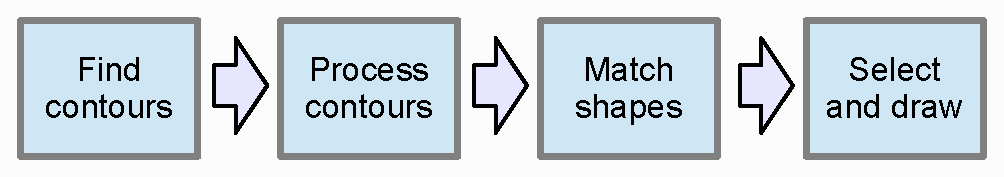
\includegraphics[width=13cm]{images/gesture_recognizer}
\caption{Block diagram of the gesture recognizer.}
\label{gesture_recognizer}
\end{figure}


\begin{itemize}
\item When the \textit{GestureRecognizer} is created, it loads the \textit{Gesture Library}. Analogously to the load of histograms, this class will load as many gestures as available, with the name format \textit{gestureX.yml}, in which \textit{X} is a number starting in 1.

\item For each hand frame, it will detect the contours with the function \textit{findContours}. This function returns a vector of closed contours.

\item Then the algorithm \textit{processes} each detected contour. It selects the biggest one (the most likely to be a hand), and it deletes \textit{extreme points}. It calculates the standard deviation, and removes the points that are very far from it. This prevents some parts of the contour that belongs to the arm of the user, and it tries to keep only those belonging to the hand. This part, thus, returns one contour.

\item For each gesture in the \textit{Gestures Library}, the selected contour is compared. In order to do this, the algorithm uses the function \textit{matchShapes} of OpenCV, which calculates the \textit{Hu Moments} of each shapes. This are seven moments that are proven to be invariable to scale, position and rotation. The function returns a similarity indicator (0 means that the shapes are the same).

\item The algorithm selects the gesture that is more similar and that has a minimum of similarity. This minimum is set by the constant \textit{MAX\_DIFFERENCE}.\\

\end{itemize}

\bigskip

Although this part is the most technical one, there are more in-deep details that are not worth explaining. If you are interested in knowing more about how this project works, or you have ideas to improve it, do not hesitate to let me know.

\label{tool}
\subsection{Histogram and gesture tool}
This tool is located in the \textit{tool} directory, and it is executed with the command \textit{./calc}. It takes a \textit{picture} of what the camera is aiming at that moment. The next step is clicking with the mouse in some region of the hand, and three windows opens:
\begin{enumerate}
\item BackProj window: it shows the result of the back projection operation. This is not very useful for the main purpose.
\item Mask window: shows what is skin. This is the most important. It is necessary to cover as much skin as possible (and as less background, of course). This can be tuned by changing the low and up threshold values. If we need to get into the mask darker part of the skin, we increase the low threshold. If we want more brighter skin, then we increase the up threshold.

It saves automatically the histogram in a file called \textit{histogram0.yml}.

\item Contours window: it shows the contour detected. It is important to set up the threshold values to to the gesture contour as well as possible. The gesture is automatically saved in a file called \textit{gesture0.yml}.
\end{enumerate}

In order to use these files in the system, they have to be copied to \textit{data/histograms} and \textit{data/gestures} respectively, and renamed (change the last number for the following one, starting in 1).


%% ========================================
%%  EVALUATION
%% ========================================

\section{Evaluation}

Developing this Computer Vision-based hand gesture recognition has been an enjoyable experience, because of the freedom to experiment with different techniques and the improving results obtained. Obviously, this algorithm is not perfect, there are a lot of improvements that can be done.\\

The most important weaknesses found are:

\begin{itemize}
\item It can be sensible to very strong illumination points (like windows or lamps). This can make the camera to auto-adjust the configuration, and then the color of the skin can change completely.
\item The contours recognized are far from being perfect, and so the detection can be wrong or delay sometimes.
\item As the number of histograms and gestures increases, the computational cost does it too.
\item Although the background accumulator can adapt to changes in the background, this takes some time.
\end{itemize}

\newpage
However, there are a lot of strengths worth mentioning:

\begin{itemize}
\item Thanks to the histogram files architecture, the illumination changes mentioned before can be handled better, cause it can use best histograms.
\item It is good to, when the application is run at the first time, not show the hand of the user, since the application stores the background at that moment. This background mask improve the results a lot.
\item The application has plenty of windows to shows the intermediate steps, which is very good for debugging.
\item As far as I tested, it works very fast (more than 25 fps at least always).
\item It is multiplatform.
\item It is modular indeed, so it is easy to incorporate in other applications. It is also easily to parallelize.

\end{itemize}

%% ========================================
%%  FUTURE WORK
%% ========================================

\section{Future work}
The more I worked on this project, the more ideas I got to improve it. Since there is a time restriction to submit this project, I could not implement all of them. Here are some of them:
\begin{itemize}
\item Optimize the code. The algorithms performs multiple image transformations, and this implies copies of long arrays several times. Once that the algorithm is completely defined, the code can be optimized to minimize the amount of copies. Copying a matrix is one of the most expensive and not useful operations, since they actually do not do anything important.

\item Implement a class \textit{Hand} that stores more information about the detected gesture. It can store position, histograms that better fits that skin in that condition, size, last gesture recognized, etc. This information can be used to make the algorithm more accurate. The seed point will be easily found, the algorithm will be faster cause it will not be necessary to calculate the skin masks for each histogram (only for those that work better in that execution), or implement succession of gestures.

\item Increase the transparency. The system itself is easy to use from other applications, but its interface can be redesigned to be more easy. For example, any application that needs to use the gesture recognizer, has to make two calls (one for \textit{HandDetectore} and another one for \textit{GestureRecognizer}). Moreover, the result interface is not clear (there is not a standard way to call the gestures recognized).

\item Make the skins and gestures library richer. The system works by loading histogram files (describing the skin color) and gesture files (describing the different contours of the gestures). It is important to provide more files describing different skin tonalities and under different light conditions, and more gestures that can be detected.

\item Port the algorithm to a mobile platform. \textit{OpenCV} works over almost any platform, so the algorithm can be theoretically run in other platforms.

\end{itemize}

\bibliographystyle{plain}  
\bibliography{report}
\end{document}

